\apendice{Documentación de usuario}

\section{Introducción}
Ene esta sección se explica como ejecutar los algoritmos de forma sencilla e intuitiva.

\section{Requisitos de usuarios}
Lo primero para que un usuario pueda ejecutar nuestro algoritmos necesitará tener instalado en el ordenador Python 3.6, a continuación se explican los requisitos necesarios:
\begin{itemize}
	\item Tener instalado una distribución de Windows instalada (solo se ha probado en Windows, pero en Linux no debería dar problemas).
	\item Instalaremos Anaconda, que es una aplicación que contiene herramientas como spyder o Jupyter, que usaremos en nuestro entorno de trabajo, esta aplicación incluye la versión de Python 3.6 requerida y nos facilita el uso de este lenguaje y la instalación de distintas librerías.
	\begin{itemize}
		\item Podemos seguir los pasos de este enlace para instalarlo \url{https://anaconda.org/anaconda/python}.		
    	\item Será necesario tenerlo instalado en la carpeta principal de nuestro usuario \textit{C:\textbackslash Users\textbackslash Usuario}.
	\end{itemize}
\item Tener el proyecto descargado o clonado con los fuentes: 

Se puede descargar a través del siguiente enlace \url{https://github.com/Tulmot/Sklearn-Multilabel.git}
\end{itemize}

\section{Instalación}
En esta parte explicaremos como instalar Anaconda de una forma sencilla por si a través del enlace no se entendió. Y también deberemos tener el proyecto ya descargado. Los pasos a seguir son:
\begin{itemize}
	\item Anaconda se puede instalar en tres sistemas operativos (Windows, Linux y Mac Os), podemos elegir el que más nos guste, este proyecto se realizó en Windows 10. Para instalarlo es tan sencillo como abrir ejecutar (tecla Windows + r), y escribir cmd, con esto se nos abrirá una ventana con la consola. Por defecto, ya estaremos en el directorio \textit{C:\textbackslash Users\textbackslash Usuario}, que es donde instalaremos la aplicación. Para ello ejecutaremos el comando \textbf{conda install -c anaconda python}, y le damos a enter. Esto puede tardar unos minutos. Una vez acabado ya tendremos instalado Anaconda en nuestra computadora.
	\item Ahora abriremos la aplicación, ya que Jupyter es una herramienta que Anaconda no trae instalada por defecto, lo único que tendremos que hacer al abrir la aplicación, es buscar la herramienta Jupyter que nos aparece al inicio y darle a \textit{install}. Con esto ya tendremos esta herramienta instalada.
	\item Como uno de los notebooks muestra árboles para que sea más visual, necesitaremos instalar también una extension llamada \textbf{Graphviz}, tendremos que hacer lo mismo que para instalar anaconda, iremos a la consola (tecla Windows + r), y escribir \textit{cmd}, cuando se haya abierto escribiremos el comando \textit{conda install python-graphviz}, pulsamos enter y se nos instalará esta extensión. 
	\item Por último, una vez descargado el proyecto, lo tendremos que descomprimir en la carpeta que deseemos.
\end{itemize}
Después de esto ya podremos ejecutar nuestro proyecto.

Hay que tener especial cuidado en cuando se realizan estos pasos tener conexión a Internet, y instalar correctamente la aplicación Anaconda en el directorio indicado.
\section{Manual del usuario}
Una vez tengamos todo instalado y configurado, como lo que queremos es ejecutar los notebooks para poder ejecutar los resultados, para poder hacerlo tenemos que abrir Jupyter para ello hay dos formas:
\begin{itemize}
	\item Abrir la consola, para ello la tecla Windows + r, se nos abre ejecutar, y hay escribimos \textit{cmd}. Allí solo tendremos que escribir \textbf{jupyter notebook} y pulsar enter.
	\item Abrir la aplicación Anaconda y desde hay lanzar el Jupyter.
\end{itemize}
Después de realizar cualquiera de las dos opciones se nos abrirá en el navegador una ventana con Jupyter, si entramos con la primera opción nos aparecerá el directorio desde el cual ejecutamos el comando \textit{jupyter notebook}, mientras que si lo hacemos con la segunda opción veremos el directorio de Documentos. Es recomendable entrar siempre desde el mismo sitio para abrir el mismo directorio, ya que ahí se alojarán nuestros notebooks. La ventana inicial que veremos, tendrá un aspecto como el que se ve en la figura \ref{fig:Jupyter}.

\begin{figure}
\centering
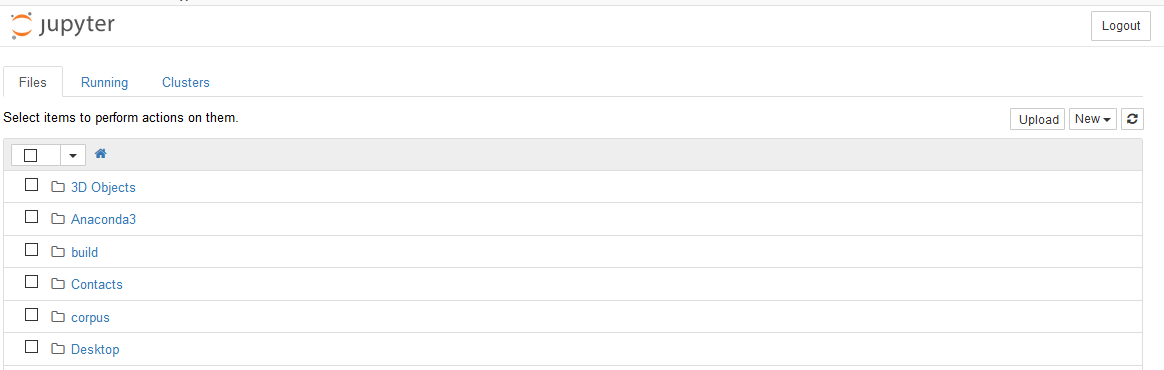
\includegraphics[width=0.95\textwidth]{Jupyter}
\caption{Ventana inicial Jupyter}
\label{fig:Jupyter}
\end{figure}

En este caso nos encontramos en el directorio del usuario \textit{C:\textbackslash Users\textbackslash Usuario}, así que veremos las carpetas y otros archivos que contenga ese directorio.

Como es la primera vez que entramos necesitaremos subir los notebooks al directorio en el que vamos a querer ejecutar nuestros notebooks. 
Para hacer esto arriba a la derecha clickaremos en el botón que pone \textit{upload}, y buscaremos donde hayamos descomprimido el proyecto descargado anteriormente. Dentro de él abriremos la carpeta \textit{src}, y seleccionaremos todos los notebooks, que son aquellos con extensión \textit{.ipynb}, también tendremos que subir el fichero \textit{flags.arff} que es un ejemplo con datos reales que usamos en el notebook \texttt{Example with real ML data set}.

Una vez subidos todos los notebooks y el fichero con datos reales. Ya podremos ejecutar los notebooks. Vamos a abrir el notebook \texttt{Example of base classifiers} y iremos explicando parte por parte como ejecutarlo, y veremos que es muy sencillo.

Para ir ejecutando cada celda en la parte superior tenemos un <<play>> que nos ira ejecutando celda a celda todas las partes.
\begin{itemize}
	\item Lo primero que veremos es el índice que podremos ver las partes en las que se divide el notebook. Podemos verlo en la siguiente figura\ref{fig:indiceJupyter}.
	\begin{figure}
	\centering
	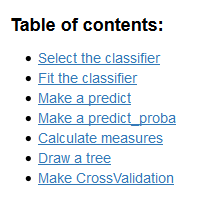
\includegraphics[width=0.3\textwidth]{indiceJupyter}
	\caption{Índice del notebook}
	\label{fig:indiceJupyter}
	\end{figure}
	\item En la siguiente parte veremos una breve explicación de que funciones va realizar el notebook, y se importan las librerías necesarias\ref{fig:importJupyter}.
	\begin{figure}
	\centering
	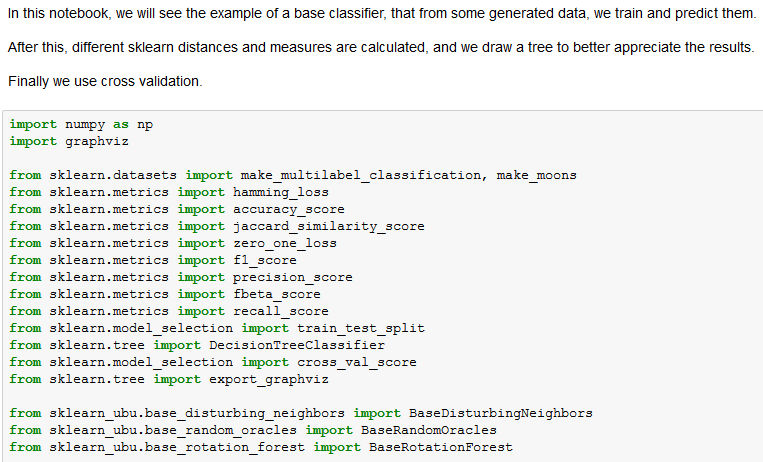
\includegraphics[width=0.95\textwidth]{importJupyter}
	\caption{Explicación e imports del notebook}
	\label{fig:importJupyter}
	\end{figure}
	\item Ahora ya empieza la parte que más afecta al usuario ya que es la que podrá modificar. Tenemos distintos parámetros que podremos modificar el conjunto de datos que crearemos\ref{fig:parametrosJupyter}.
	\begin{figure}
	\centering
	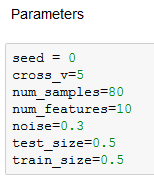
\includegraphics[width=0.25\textwidth]{parametrosJupyter}
	\caption{Parámetros que se pueden modificar}
	\label{fig:parametrosJupyter}
	\end{figure}
	\begin{itemize}
		\item Seed: Este parámetro lo que hace es que los valores que generemos no sean aleatorios.
		\item Cross\_v: Este parámetro lo usaremos para validación cruzada, es el número de partes que dividiremos el conjunto de datos a la hora de hacer el cruce.
		\item Num\_samples: Es el número de instancias/filas que queremos que tenga nuestro conjunto de datos.
		\item Num\_features: El número de características/columnas que queremos que tenga nuestro conjunto de datos.
		\item Noise: Es la desviación que tendrán los datos.
		\item Test\_size: Es el porcentaje del conjunto de datos que utilizaremos para testear.
		\item Test\_train: Es el porcentaje del conjunto de datos que utilizaremos para entrenar.
	\end{itemize}
	\item Según el conjunto de datos que queremos crear si es Single-Label o Multi-Label, deberemos ejecutar solo la celda deseada. Posteriormente se divide el conjunto de datos en una parte de entrenamiento y otra de pruebas\ref{fig:crearDatosJupyter}.
	\begin{figure}
	\centering
	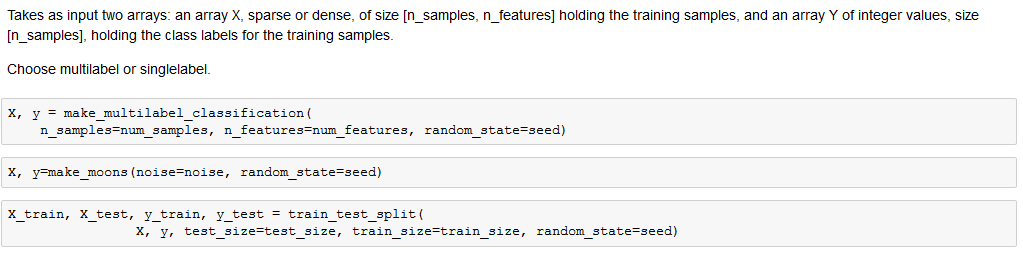
\includegraphics[width=0.95\textwidth]{crearDatosJupyter}
	\caption{Seleccionar Single-Label o Multi-Label}
	\label{fig:crearDatosJupyter}
	\end{figure}
  	\item Ahora tenemos tres clasificadores para elegir, como en el paso anterior solo debemos ejecutar la celda del clasificador que deseamos usar\ref{fig:classifierJupyter}.
  	\begin{figure}
	\centering
	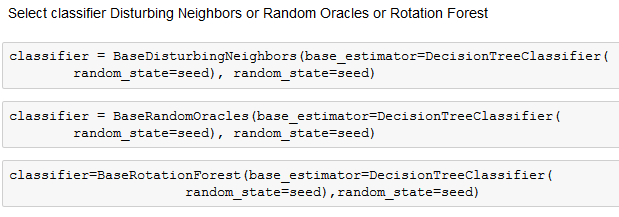
\includegraphics[width=0.8\textwidth]{classifierJupyter}
	\caption{Seleccionar el clasificador}
	\label{fig:classifierJupyter}
	\end{figure}
	\item En la siguiente figura\ref{fig:trainJupyter} se entrena el conjunto de datos con el clasificador seleccionado.
  	\begin{figure}
	\centering
	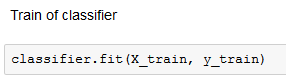
\includegraphics[width=0.4\textwidth]{trainJupyter}
	\caption{Entrenamos el clasificador}
	\label{fig:trainJupyter}
	\end{figure}
	\item Una vez el clasificador entrenado ya podemos predecir con él\ref{fig:predictJypyter}.
  	\begin{figure}
	\centering
	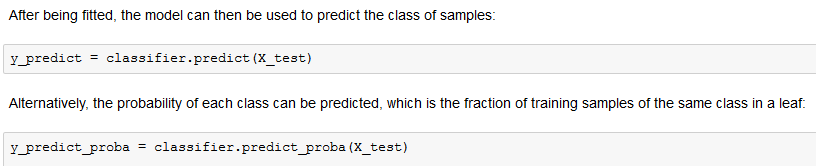
\includegraphics[width=0.95\textwidth]{predictJypyter}
	\caption{Predecimos con el clasificador entrenado}
	\label{fig:predictJypyter}
	\end{figure}
	\item Ya que hemos acabado de entrenar y predecir nuestro conjunto de datos ahora queremos ver algunas medidas para ver los resultados\ref{fig:medidasJupyter}.
  	\begin{figure}
	\centering
	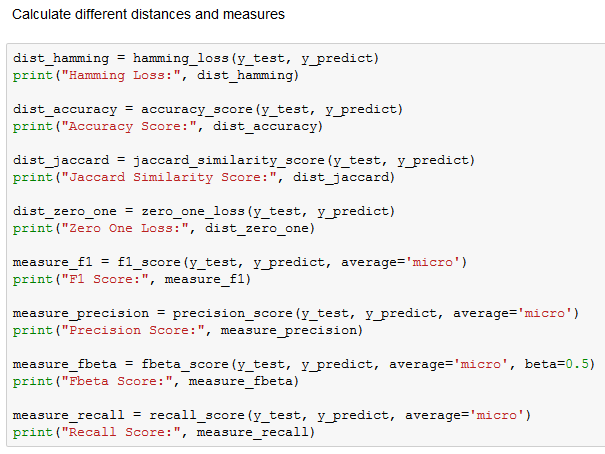
\includegraphics[width=0.8\textwidth]{medidasJupyter}
	\caption{Resultados}
	\label{fig:medidasJupyter}
	\end{figure}
	\item Para acabar dibujamos un árbol de nuestro clasificador entrenado para que sea mas visual\ref{fig:arbolJupyter}.
  	\begin{figure}
	\centering
	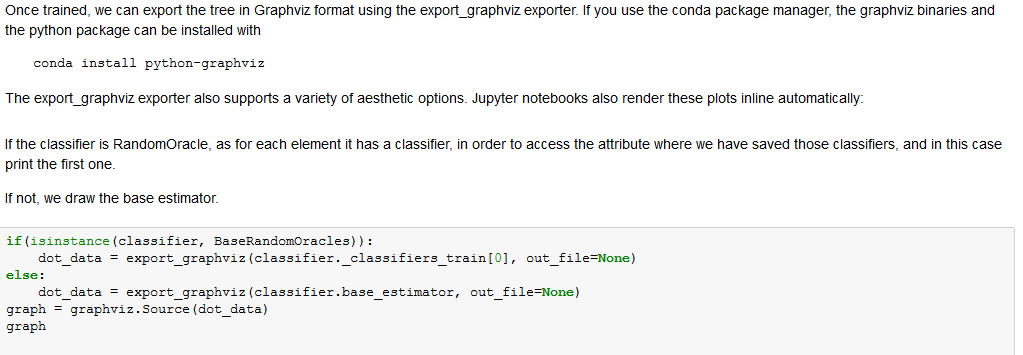
\includegraphics[width=0.95\textwidth]{arbolJupyter}
	\caption{Árbol de clasificador entrenado}
	\label{fig:arbolJupyter}
	\end{figure}
\end{itemize}

Los demás notebooks son relativamente parecidos por lo que se entiende que no hace falta explicar como se ejecutan, los únicos que son algo distintos son el de notebook de \textit{Graphics} y el de \textit{DT vs ensembles}, en el primero se muestran unas gráficas de como divide el conjunto de datos cada algoritmos, así podemos ver como funciona internamente. En el segundo es una comparativa en el que se usan cinco conjuntos de datos y se compara el clasificador \texttt{DecisionTreeClassifier} con los tres algoritmos realizados \texttt{DisturbingNeighbors}, \texttt{RandomOracles} y \texttt{RotationForest}, para ver como son mejores, se ve una tabla con la precisión de cada clasificador para cada conjunto de datos.